%!TEX root = ../../Main.tex
\graphicspath{{Chapters/Test/}}
%-------------------------------------------------------------------------------


\section{I2C kommunikation}
Til at starte med havde gruppen ikke planer om at inkorporere I2C i NSS, da den simple løsning var at have både TFT skærmen og Color Sensoren sat til samme Arduino. Dette viste sig ikke at kunne lade sig gøre, da skærmen og sensoren delte nogle pins, hvilket gjorde at systemet ikke fungerede. Desværre kunne vi ikke bruge andre pins til sensoren, da de to pins der er at vælge imellem begge sad i vejen for skærmen. Derfor valgte gruppen at splitte systemet op og anvende I2C. På grund af denne ekstra arbejsbyrde, blev SD kort implementationen nedprioriteret.



\subsection{I2C master}
Masteren blev valgt implementeret på TFT display modulet, da det ikke ville give mening at lade sensor modulet sende kommandoer til display modulet. Istedet for sendes der en char fra slaven, som repræsenterer en farve.

Før masteren kan bruges skal den først initiereres. Dette sker ved at sætte bestemte dataregistre op rigtigt. Først bestemmer man hvilken clock SCL skal have. SCL kan udregens på følgende måde:

\begin{equation}
SCL= \frac{CPU}{16+2(TWBR)*4^{TWPS}} 
\end{equation}

Gruppen har valgt at en clock på 500KHz. De eneste krav til clokcen er at den er 16 gange lavere end slavens cpu clock, ifølge megea 2560 datablad. Da slaven kører med 16MHz, opfylder den det krav. 



\begin{figure}[H]
	\centering
	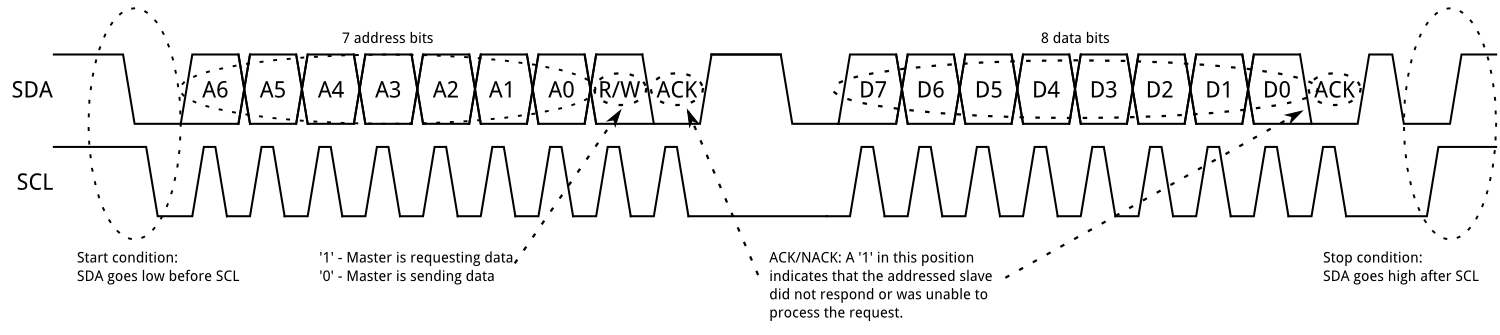
\includegraphics[width = 450pt]{Img/I2CTiming.png}
	\caption{I2C timing diagram}
	\label{fig:I2CTIming}
\end{figure}


Til udviklingen af masteren har et timing diagram over I2C protokollen, se \autoref{fig:I2CTIming}, været utrolig nyttig. Ved hjælp af dette diagram har gruppen kunne sende korrekte beskeder over I2C. 

For at have en så overskuelig kode som overhovedet muligt, er der blevet lavet funktioner der kan generere ACK, NACK, WAIT, START og STOP. Disse funktioner er så brugt i vores i2c\_master\_receive funktion. Et Kodeudsnit af denne funktion kan findes nedenunder:

\newpage

\begin{lstlisting}
i2c_master_start();
while(transfer && i < 250)
{
	//usart_transmit(twi_master_status());
	switch (i2c_master_status())
	{
		// Start condition has been transmitted
		case 0x08:
		// Contact slave and enter master transmitter mode
		TWDR = address_r;
		i2c_master_ack();
		i2c_master_wait();
		break;
		
		// SLA+R has been transmitted and acked
		case 0x40:
		i2c_master_nack();
		i2c_master_wait();
		break;
		
		// Data byte has been received and acked
		case 0x50:
		//SendChar('A');
		data = TWDR;
		transfer = 0;
		break;
		
		// Data byte has been received and nacked
		case 0x58:
		//SendChar('B');
		data = TWDR;
		transfer = 0;
		break;
	}
	i++;
}
i2c_master_stop();
\end{lstlisting}

Som det ses i koden bliver i2c\_master\_status() hele tiden tjekket på, for at finde ud af om slaven reagerer på nogle af kommandoerne fra masteren. Status funktion tjekker TWSR registeret og AND'er det med 0xF8, for at sætte de tre sidste bits til 0. I mega 2560 datablad kan der findes en tabel over hvad de forskellige status koder står for. I kode udsnittet står de som kommentarer over hver case.

\subsection{I2C slave}
Ligesom masteren skal slave også initialiseres, ved at sætte nogle bestemte dataregistre op. TWAR registeret bestemmer slavens adresse, i vores tilfælde er den sat til 40. TWCR registeret bestemmer hvilken slave mode den skal sættes i, i vores tilfælde er det slave transmitter mode. Det vil sige at slaven kun skal kunne sende data til masteren, og ikke omvendt. 

Når slaven er sat op i transmitter mode, bliver der gjort brug af et interrupt, der når i2c interfacet bliver brugt. Når et interrupt bliver triggered, køres vores interrupt rutine, som kan ses nedenunder:

\begin{lstlisting}
if(i2c_slave_addressed())
{
	
	switch(i2c_slave_status())
	{
		
		case 0x60:
		i2c_slave_ack();
		break;
		
		case 0x80:
		SendChar('A');
		data = TWDR;
		i2c_slave_ack();
		transfering = 0;
		break;
		
		case 0xA8:
		TWDR = dataToSend; //data send to master
		i2c_slave_ack();
		break;
		
		// Last byte sent by master
		case 0xC0:
		transfering = 0;
		i2c_slave_ack();
		break;
	}
}
\end{lstlisting}

Interrupt rutinen minder meget om masterens receive funktion. Den tjekker hele tiden på status registeret(TWSR), for at holde styr på hvor langt den er i I2C processen. dataToSend indeholder en char med information om hvilken farve color sensoren har opfanget. 



\subsection{Test}

Billede af logic analyzer! og forklarende tekst

